\documentclass[a4paper, 11pt, titlepage]{article}
\usepackage[utf8]{inputenc}
\usepackage[english]{babel}
\usepackage[]{parskip}
\usepackage{graphicx}
\usepackage{paralist} % compactitem
\usepackage{csquotes}
\usepackage[
  style=ieee,
  citecounter,
  labelnumber,
  backend=biber,
  bibencoding=utf8,
  sorting=none
]{biblatex}
\addbibresource{references.bib}
\usepackage{wrapfig}
% Custom commands
\newcommand{\figRef}[1]{Figure \ref{#1}}
\newcommand{\tabRef}[1]{Table \ref{#1}}
\newcommand{\eqRef}[1]{(\ref{#1})}

\title{EECE6036 - Homework 1}
\author{Wayne Stegner}
\date{\today}

\begin{document}
  \maketitle
  \section{Problem 1}
  \subsection{Problem Summary}
  \par This problem involves simulating a single neuron as defined by the
  Izhikevich model \cite{Izhikevich2003}.
  This neuron is defined by the following differential equations:
  \begin{equation}
    \frac{\partial v}{\partial t} = 0.04v^{2} + 5v + 140 - u + I(t)
    \label{eq:dv}
  \end{equation}
  \begin{equation}
    \frac{\partial u}{\partial t} = a(bv - u)
    \label{eq:du}
  \end{equation}
  \begin{equation}
    if v \geq 30; v = c, u = u + d
    \label{eq:cond}
  \end{equation}
  \par The neuron is simulated in the \textit{Regular Spiking} configuration
  ($a=0.02$, $b=0.25$, $c=-65$, $d=6$), described in
  \cite{Izhikevich2003,Izhikevich2004}, with a range of DC synaptic currents,
  $I(t)$, over 1000 ms with a time step of 0.25 ms.
  Each trial uses a static value of $I(t)$ ranging from $I(t)=0$ to $I(t)=20$
  with a step of 0.5.
  The purpose of this problem is to measure the membrane potential of the neuron, as well as
  the mean spiking rate for each value of $I(t)$.
  \subsection{Results}
  \begin{wrapfigure}{r}{0.5\textwidth}
    \centering
    \vspace{-44pt}
    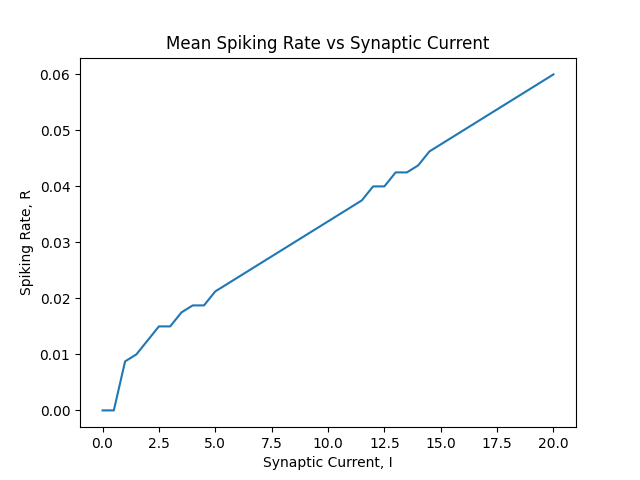
\includegraphics[width=0.48\textwidth]{images/spike_rate_single.png}
    \vspace{-10pt}
    \caption{
      Mean spiking rate as a function of synaptic current of a single neuron.
    }
    \vspace{-22pt}
    \label{fig:rSingle}
  \end{wrapfigure}
  \figRef{fig:rSingle} shows the mean spiking rate plotted as a function of the
  synaptic current.
  Spiking rate is calculated by averaging the number of spikes per ms over the
  last 800 ms of each simulation.
  \figRef{fig:vSingle} shows the membrane potential plotted over 1000 ms for
  various input currents.
  \begin{figure}[ht]
    \centering
    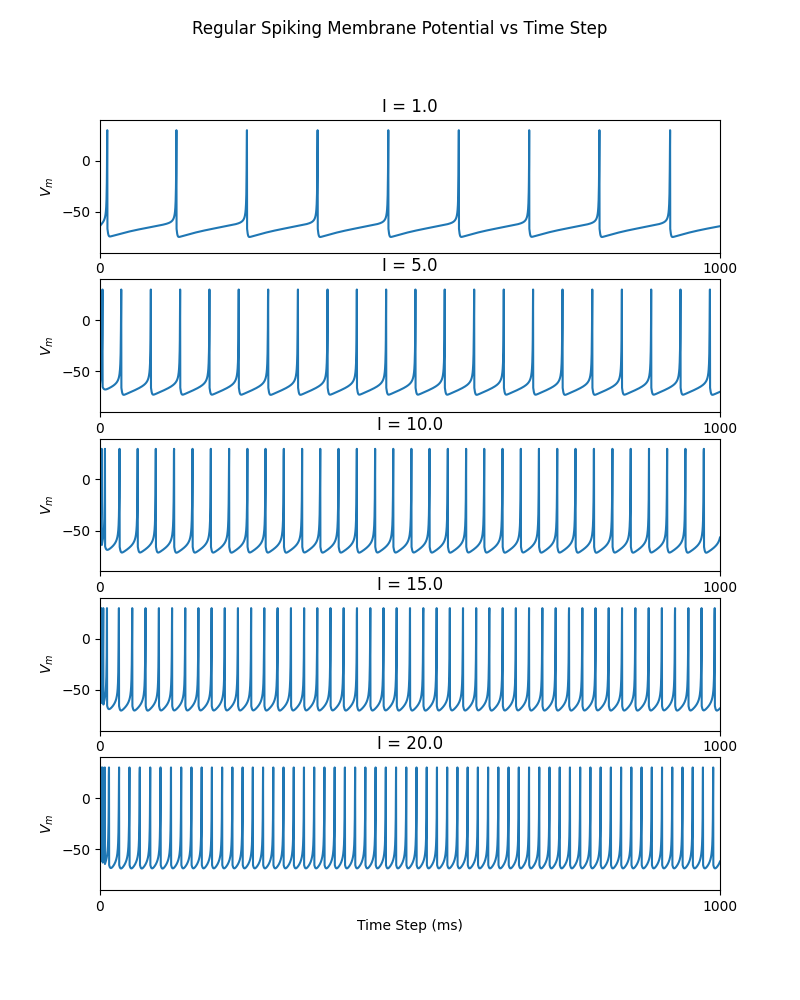
\includegraphics[width=0.8\textwidth]{images/v_mem_plot_single.png}
    \vspace{-20pt}
    \caption{
      Membrane potential as a function of time for various input currents for a
      single neuron.
    }
    \label{fig:vSingle}
  \end{figure}
  \subsection{Discussion}
  \par In \figRef{fig:rSingle}, the mean spiking rate is roughly a linear
  function of the input current.
  The spiking rate is more visually illustrated in \figRef{fig:vSingle}.
  When the simulation starts, there is an initial short burst of spikes, which
  then settles out into a steady sequence of spikes.
  This initial burst is why the first 200 ms of simulation are discarded before
  calculating the mean spiking rate.
  Effectively, this simulation demonstrates the use of a \textit{Regular
  Spiking} neuron to translate a DC input into a spike train, where the higher
  DC level translates to a higher frequency spike train.
  \subsection{Conclusion}
  In this problem, a simulation of a single \textit{Regular Spiking} neuron
  using the Izhikevich model \cite{Izhikevich2003} with various DC input levels
  is presented.
  The resultant membrane potential plots in \figRef{fig:vSingle} reflect the
  intended behaviour described by Izhikevich \cite{Izhikevich2003,
  Izhikevich2004}.
  This work shows that a semi-realistic artificial neuron can be simulated
  using little computational overhead.
  \pagebreak
  \section{Problem 2}
  \subsection{Problem Summary}
  This problem builds upon the first, involving the simulation of a simple
  network of two neurons with parameters as described in Problem 1.
  Neuron A gets the input $I_{A} = 5$ and outputs the spike train $y_{A}$,
  while neuron B gets input $I_{B}(t)$ and outputs the spike train $y_{B}$.
  The system can be defined as:
  \begin{equation}
    I_{B}(t) = I_{B} + w_{BA} * y_{A}(t)
    \label{eq:IB}
  \end{equation}
  \begin{equation}
    y_{i}(t) = 1 \quad if \quad v_{i} > 30, \quad else \quad y_{i} = 0
    \label{eq:spiketrain}
  \end{equation}
  where $w_{BA}$ is the weight between neurons A and B and is fixed at 10.
  Similarly to Problem 1, each trial uses a static value of$I_{B}$ ranging
  from 0 to 20 with a step of 5.
  The purpose is to measure the membrane potential of the neuron, as well as
  the mean spiking rate for each value of $I_{B}$.
  \subsection{Results}
  \begin{wrapfigure}{r}{0.5\textwidth}
    \centering
    \vspace{-40pt}
    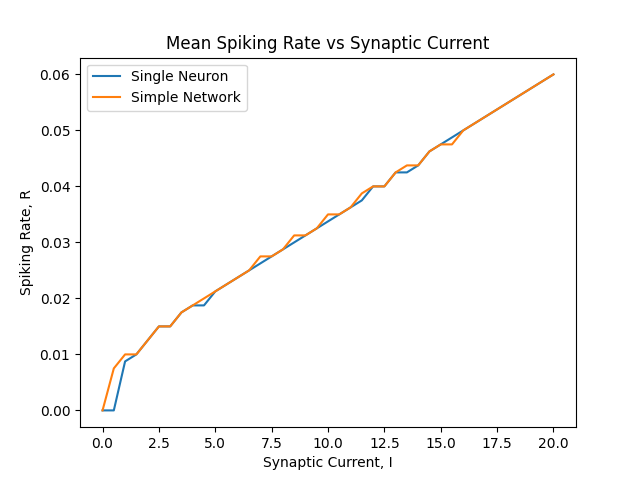
\includegraphics[width=0.48\textwidth]{images/spike_rate_network.png}
    \vspace{-10pt}
    \caption{
      Mean spiking rate as a function of synaptic current of a single neuron
      (blue) vs the simple network (orange).
    }
    \vspace{-10pt}
    \label{fig:rNetwork}
  \end{wrapfigure}
  \figRef{fig:rNetwork} shows the mean spiking rate plotted as a function of
  the synaptic current for both the single neuron in Problem 1 and the network
  from this problem.
  Spiking rate is calculated by averaging the number of spikes per ms over the
  last 800 ms of each simulation.
  \figRef{fig:vNetwork} shows the membrane potential is plotted over 1000 ms
  for various values of $I_{B}$.
  \begin{figure}[ht]
    \centering
    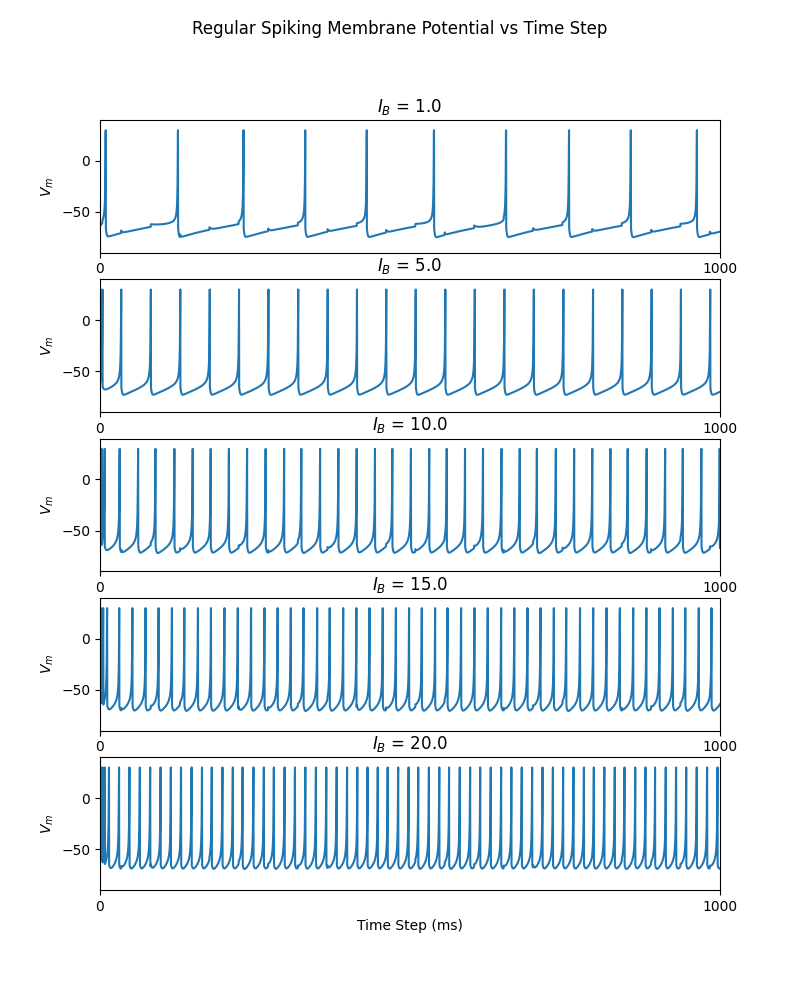
\includegraphics[width=0.8\textwidth]{images/v_mem_plot_network.png}
    \vspace{-20pt}
    \caption{
      Membrane potential as a function of time for various input currents for a
      simple network.
    }
    \label{fig:vNetwork}
  \end{figure}
  \subsection{Discussion}
  In \figRef{fig:rNetwork}, the mean spiking rate of the network exhibits
  similar characteristics as the single neuron, with both of them roughly
  a linear function of the input current.
  While there are slight fluctuations between the two plots, the overall trend
  is identical.
  In \figRef{fig:vNetwork}, the spiking rate looks very similar to those shown
  in the single neuron in \figRef{fig:vSingle}.
  When $I_{B} = 1$, there are slight perturbations which can be observed as the
  neuron gradually approaches its spike.
  They can be seen in most of the values of $I_{B}$, but they are the most
  evident when $I_{B} = 1.0$.
  These perturbations are caused by the spike train generated by neuron A, but
  they do not seem to have an impact on the overall behaviour of neuron B.
  \subsection{Conclusion}
  In this problem, a simulation of a network of two \textit{Regular Spiking}
  neurons using the Izhikevich model \cite{Izhikevich2003} with various DC
  input levels is presented.
  The resultant membrane potential plots in \figRef{fig:vNetwork} do not
  deviate much from the results of a single neuron in \figRef{fig:vSingle},
  and the mean spiking rate in \figRef{fig:rNetwork} shows how similar the
  behaviour of the network of neurons is to the single neuron.
  The perturbations induced by neuron A were quickly dissipated in neuron B,
  which suggests that in order for artificial spiking neurons to impact each
  other, either a more dense spike train is needed as an input into neuron B,
  or neuron B should be tuned to not dissipate incoming spikes as quickly.
  \pagebreak
  \printbibliography
\end{document}
